\subsection{Asynchronous Programming With \netstar: the IDS Example}
\label{IDSexample}

\begin{comment}
\begin{figure}[!t]
\centering
\begin{lstlisting}[style=CStyle]
void run_async_flow_manager() {
  repeat([this]{
    return _manager.on_new_async_flow().then([this]() {
      auto af = _manager.cur_async_flow();
      do_with(malware_detector(std::move(af)),
        [](malware_detector& nf){
          nf.events_registration();
          return nf.run();
        });
      return stop_iteration::no;
    });
  });
}
future<> malware_detector::run() {
  return _af.register_loop_fn([this](){
    ...
    if(_af.preprocessor.on_file_hash_event()) {
      // Get file hash from preprocessor.
      auto _hash=_af.preprocessor.get_file_hash();
      return _db.lookup(_hash).then([this](db_res res){
        if(malware_detected_in_db(res)){
          // File hash is stored in local database.
          record_detected_malware();
          return ready_future(action::drop);
        }
        // File hash is not stored in local database.
        string name=build_up_name(_hash);
        return _dns.query(name).then([this](dns_res res){
            if(malware_detected_in_mhr(res)){
              // File hash is presented in MHR.
              record_detected_malware();
              return ready_future(action::drop);
            }
            // File passes malware detection.
            return ready_future(action::forward);
        });
      }).then_wrapped([this](future<action> f){
        try {
          return f.get();
        }
        catch(...) {
          // Either database or DNS query timeouts.
          record_malware_detection_error();
          return ready_future(action::drop);
        }
      });
    }
    ...
  });
}
\end{lstlisting}
\caption{Malware detector implemented using \netstar.} %It uses the same detection method as in Bro.}
\label{fig:netstar-code-sample}
\end{figure}
\end{comment}


\begin{figure}[!h]
\centering
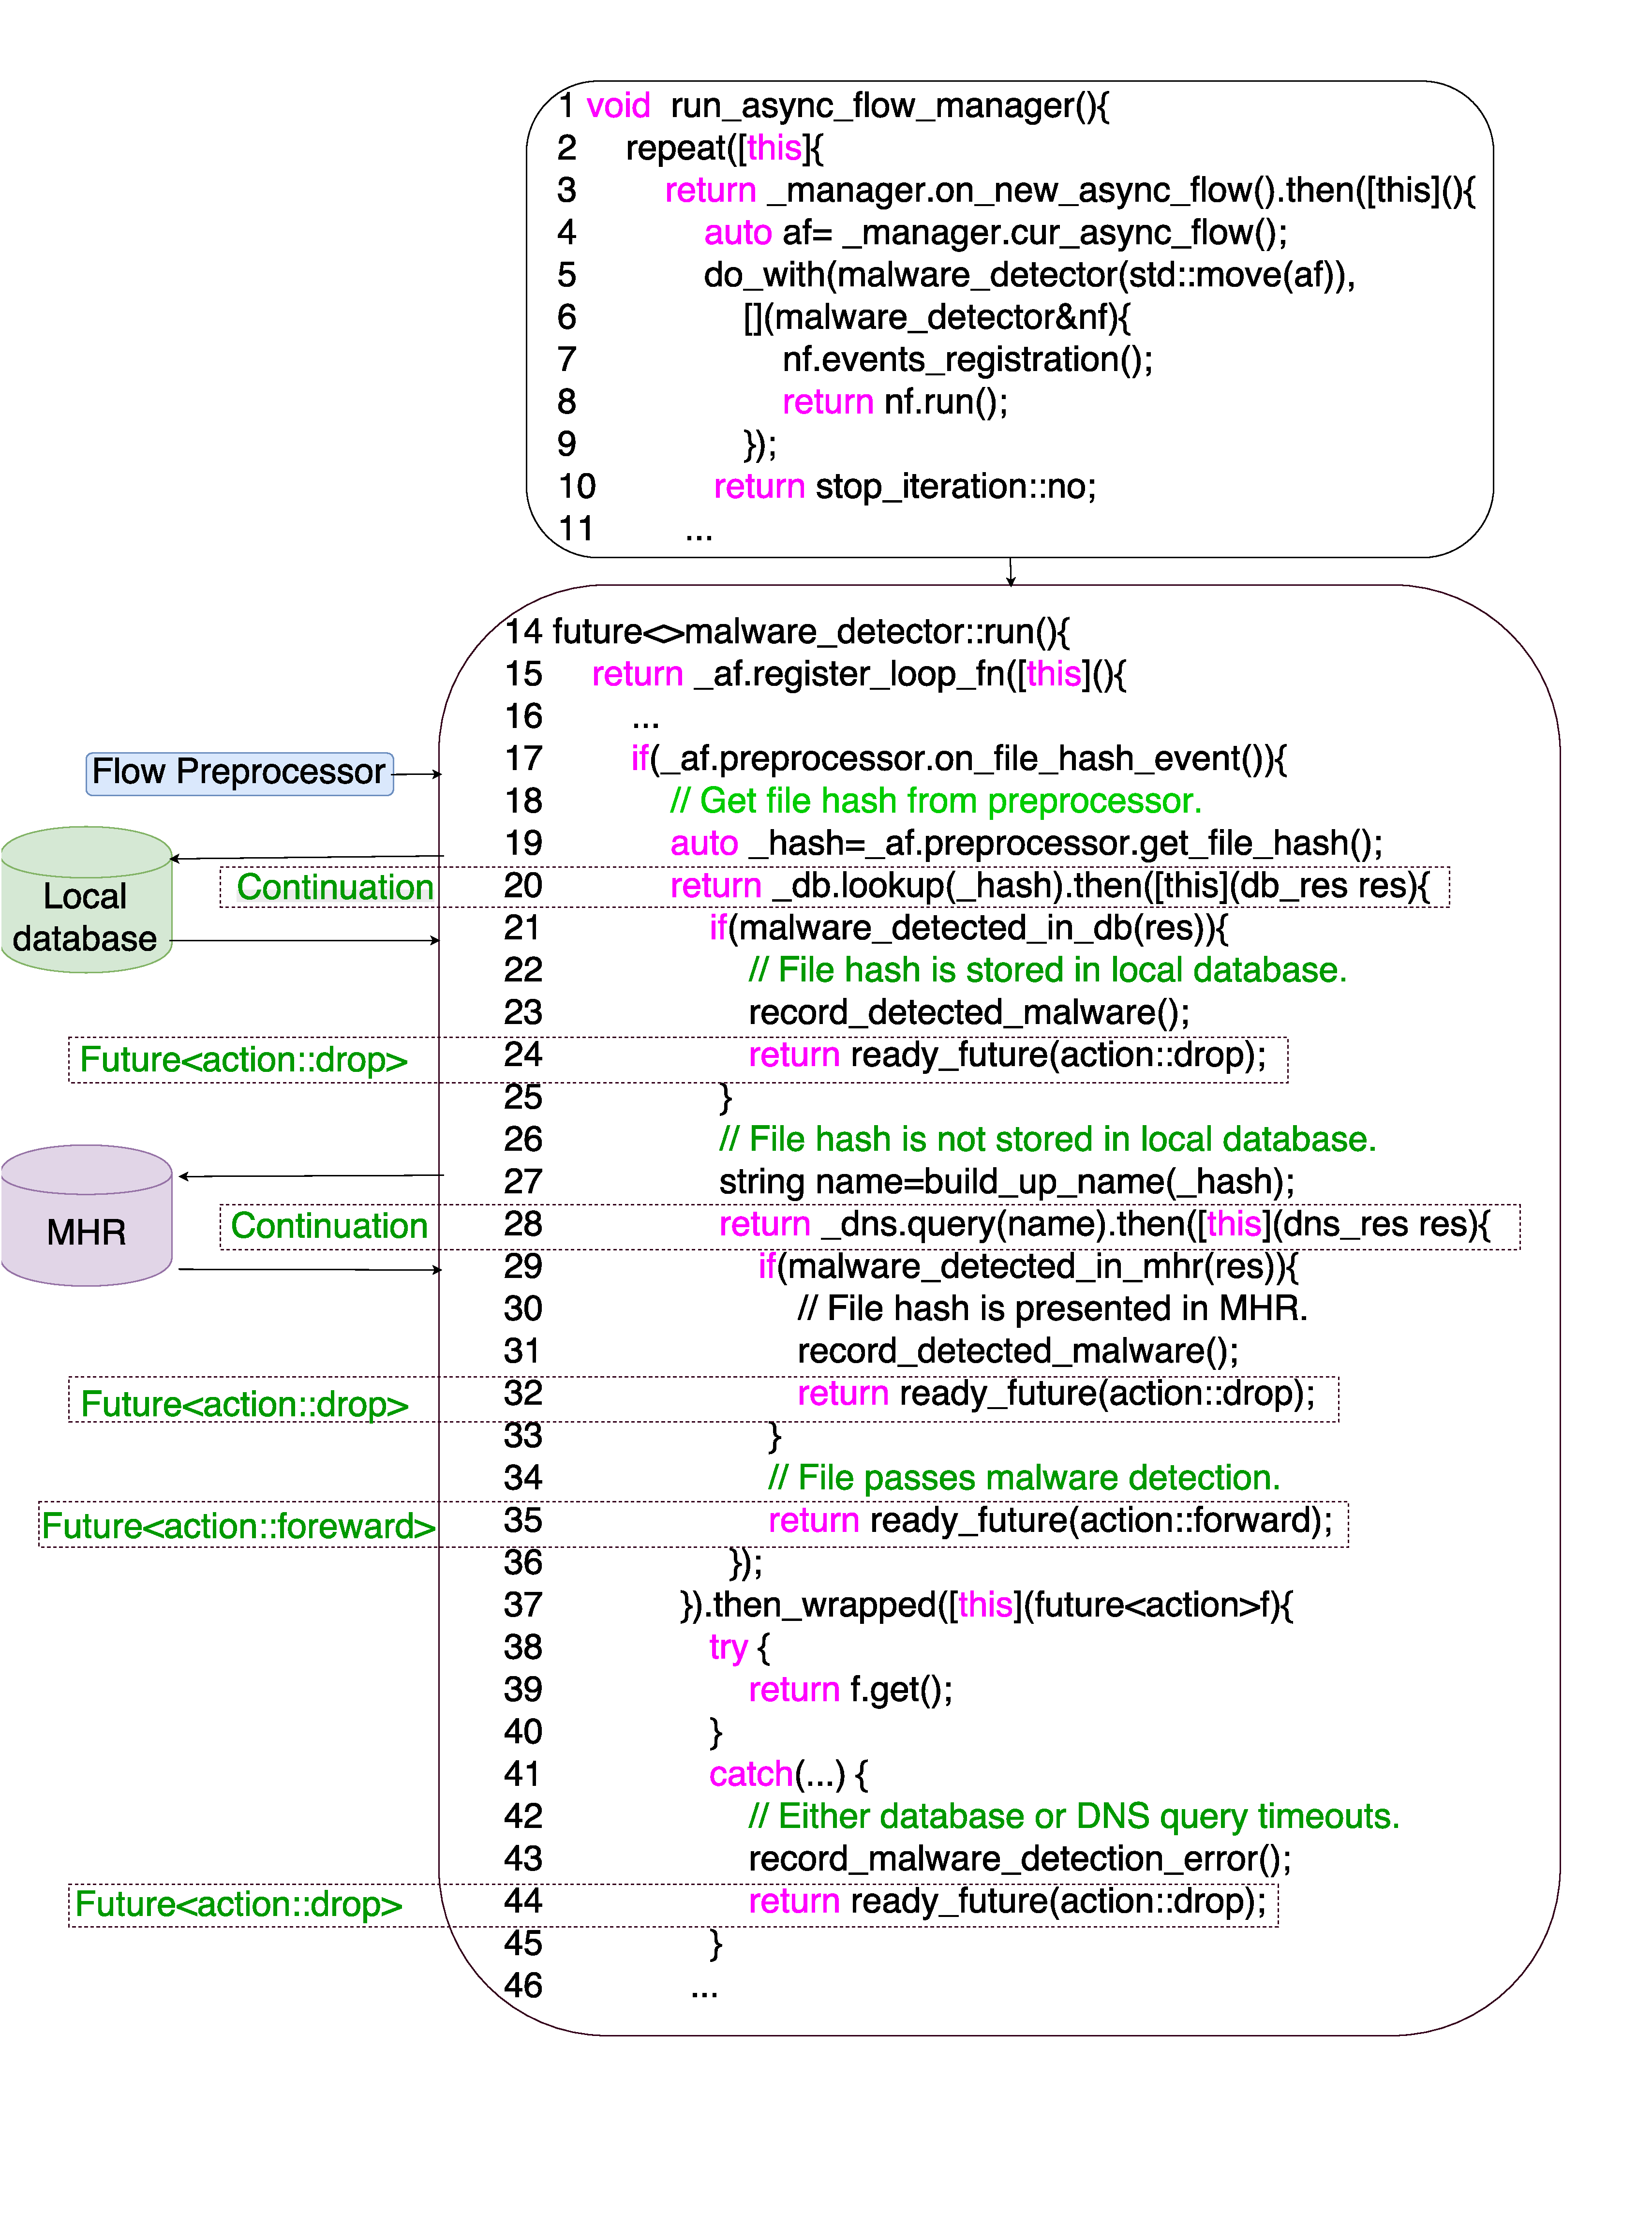
\includegraphics[width=\columnwidth]{chap-netstar/figure/netstar_code_graph.pdf}
\caption{Malware detector using \netstar.}
\label{fig:netstar-code-sample}
\end{figure}


Now we present the implementation of a malware detector using the async-flow interface designed above, which achieves similar functionalities as the Bro example in Sec.~\ref{sec:bro}. %, except the following: In Bro's implementation, when some malware is detected, only the event is logged %, and the packets are still forwarded to the next hop
%(mainly due to their implementation choice of decoupling the malware detection process from the packet processing loop); our code works in an in-line mode, that when it detects some malware in a flow, it drops all the subsequent flow packets and stops the flow from reaching the next hop.

Our code sketch is given in Fig.~\ref{fig:netstar-code-sample}. \lstinline[style=InlineStyle]{run_async_flow_manager} runs the async-flow manager, which constantly checks (lines 2-3) incoming new flows. If a new TCP flow has arrived, %(indicated by a new flow 5 tuple in a received packet),
a new async-flow object is created to handle the flow (line 4), and a malware detector object is associated with the new async-flow object (line 5). The malware detector object expresses its interest in the file hash event by registering this event %to the async-flow object
(line 7). The core processing logic of the malware detector is then registered with the async-flow object by calling \lstinline[style=InlineStyle]{register_loop_fn} (line 15),
%The malware detector is then started by calling \lstinline[style=InlineStyle]{run} (line 8). \chuan{explain what happens to existing flows. I do not see where in the code handling of existing flow is done}.
%In \lstinline[style=InlineStyle]{run}, core processing logic of the malware detector is registered with ...\chuan{registered with the async-flow object? change the name of loop in the code} (line 15), % does nothing but to register a loop function as in line 17,
which is carried out upon occurrence of the file hash event.


First, the preprocessor %to handle each received packet in the flow is a TCP payload reassembler, which
reconstructs the TCP byte stream as it receives each new flow packet (code omitted from Fig.~\ref{fig:netstar-code-sample}). After processing a packet, if the preprocessor detects a newly transmitted file, it calculates the hash value of this file and raises a the file hash event. % as discussed in Sec.~\ref{sec:bro}.
In case that the preprocessor fails to detect a transmitted file, it only raises a packet arrival event, which is ignored by the core processing logic, % registered by the malware detector object,
 and the packet is forwarded out directly.

After a file hash event is generated (line 17), the core processing logic %is called to handle this event
(lines 19-37) implements similar malware detection steps as discussed in Sec.~\ref{sec:bro}.
A database query is initiated by \lstinline[style=InlineStyle]{_db.loopkup} and a future object is obtained which contains the database response (line 20); a continuation function is appended for checking the query result. If some malware is detected, the packet is immediately dropped by returning a future object containing a drop action (line 24). Otherwise, it moves on to query the MHR with a DNS query using \lstinline[style=InlineStyle]{_dns.query} (line 28). The continuation function appended to the future containing the DNS query response checks the query result. If some malware is detected, the continuation function returns a future object containing a drop action as well (line 32); otherwise, the continuation function returns a future object containing a forward action (line 35). The code from line 38 to line 47 handles potential exceptions generated during database or DNS queries, as a continuation function appended to the returned future object.

%If a malware is detected, the malware detector records this detection by calling \lstinline[style=InlineStyle]{record_detected_malware()} (line 23 and 31). The \lstinline[style=InlineStyle]{record_detected_malware()} function asks the async-flow object to deliver all the packet arrival event to the malware detector object, which drops all subsequent packets by default.


\noindent\textbf{Comparison.} The malware detector implemented with \netstar~has the following advantages over that in Fig.~\ref{fig:code-sample}.
(1) {\em Simplified Implementation.} The malware detection process can be concisely implemented in \netstar~using only 18 lines of code (lines 19-37). Our code mimics the sequential execution of database and DNS queries within a single function, instead of spreading the execution flow across multiple functions.
(2) {\em Simplified Context Management.} In our code, the context information is put directly into the malware detection object. Different continuation functions (lines 15, 20, 28, 37) can easily visit the saved context by capturing a pointer (\lstinline[style=InlineStyle]{this}) to the malware detection object. Since the malware detector object is only destroyed when the packet processing loop stops running (line 5), the above code guarantees that the malware detector object is always alive when the continuation functions are being called.
(3) {\em Consolidated Error Handling.} Instead of defining two error handling functions, our implementation consolidates the error handling logic within a single continuation function (lines 38-47). %, eliminating redundant definitions.
The programmer can be more focused on the core NF processing logic, while simply chaining another continuation function at the end for handling all errors that might be generated from the core code.

%\chuan{`this' represents the packet context?}
%we capture a pointer to the malware detection object (\lstinline[style=InlineStyle]{this} shown in Fig.~\ref{fig:netstar-code-sample}) within different continuation functions (line 15, 20, 28, 37)
%. By putting all relevant context information within the malware detection object, NetStar simplifies context management
%The design of the async-flow interface uses reference counting \chuan{I do not see reference counting mentioned in  async-flow interface} to guarantee that when the continuation function is called, the malware detection object is never destroyed \chuan{clarify how is the related to context management}.

%{\em Support of Inline Mode.} The Bro code in Fig.~\ref{fig:code-sample} does not run in in-line mode. The malware detection process is decoupled from the packet processing loop of Bro. So that when the malware is detected, Bro can only log the event, instead of stopping the flow from reaching the target. Our async-flow interface design guarantees that while an asynchronous operation is going on, the packet can be buffered without releasing. When the asynchronous operation finishes, the async-flow interface determines whether to forward the packet or now by checking the value returned in the future object (line 24,32,35,44). In this way, we can effectively implement a malware detector that runs in inline mode to better protect the backend.
